\documentclass[../Main.tex]{subfiles}

\graphicspath{{\subfix{../Figures_and_Tables/}}}
 
\begin{document}

\newpage
\begin{figure}[t]
	\begin{center}
	\caption{\label{fig:nh_con_map} \centering Nursing Home Certificate-of-Need Regulation in the United States}
    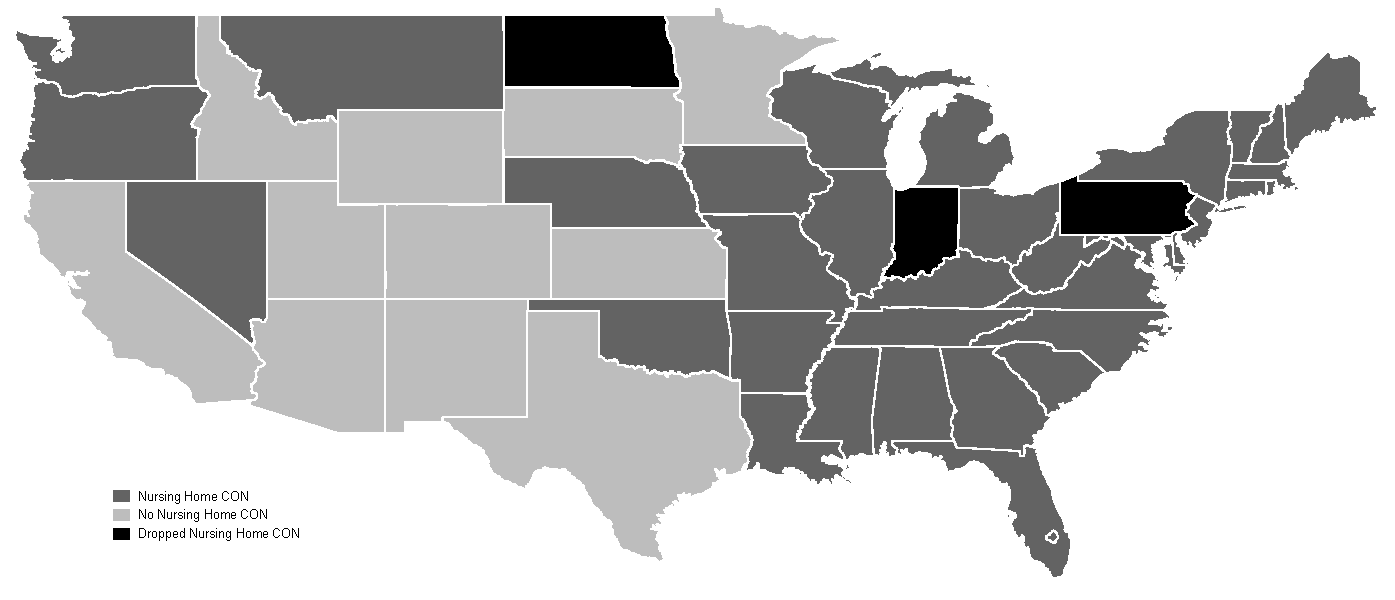
\includegraphics[width=\textwidth,keepaspectratio]{CON_Map.pdf}
    \end{center}
    \footnotesize
		\textit{Notes}: This figure shows which states dropped NH-CON regulations during our sample period (black), and which states did (dark gray) and did not (light gray) have NH-CON regulations during our sample period. All of the states that had NH-CON during our sample period except Connecticut and Louisiana, both of which adopted NH-CON during the sample period, were included in our donor pool of potential controls when finding synthetic matches for the states that dropped NH-CON. Data source: American Health Planning Association (AHPA), compiled by \citet{stratmann2014certificate}, and the National Conference of State Legislatures.
\end{figure}
\clearpage


\newpage
\begin{figure}[t]
    \begin{center}
	\caption{\label{fig:model_graph} The Effect of NH-CON on Nursing Home Quality}
	\begin{tikzpicture}[scale=1]
    % Axis
    \coordinate (y) at (0,9);
    \coordinate (x) at (10,0);
    \draw[<->] (y) node[above] {$c_z'(z_i)$} -- (0,0) --  (x) node[right] {$z_i$};
    \node [above] at (0,9.6) {$MB(z_i)$,};
    % Draw help grid
    %\draw[step=10mm, lightgray] (0,0) grid (10,10); 
    % define some coordinates
    %\path
    \coordinate (cstart) at (0,0);
    \coordinate (cend) at (10,8);
    \coordinate (mb0start) at (0,2.5);
    \coordinate (mb0end) at (10,6);
    \coordinate (mb1start) at (0,1.5);
    \coordinate (mb1end) at (10,5);
    % Draw the lines
     \draw[thick, name path=c] (cstart) to[bend right = 30] (cend) node[right] {$c_z'(z_i)$};
     \draw[thick, name path=mb0] (mb0start) to[bend left = 15] (mb0end) node[right] {$MB^{No~CON}(z_i)$};
     \draw[thick, name path=mb1] (mb1start) to[bend left = 15] (mb1end) node[right] {$MB^{CON}(z_i)$};
     \path[name intersections={of=c and mb0, by=eq0}];
     \draw[black,fill] (eq0) circle[radius = 2pt];
    \draw[thick, dotted] (eq0) -- (eq0 |- 0,0) node[below,xshift=.5cm]{$z_i^{*No~CON}$};
    \path[name intersections={of=c and mb1, by=eq1}];
     \draw[black,fill] (eq1) circle[radius = 2pt];
    \draw[thick, dotted] (eq1) -- (eq1 |- 0,0) node[below,xshift=-.2cm]{$z_i^{*CON}$};
\end{tikzpicture}\\
		\end{center}
		\footnotesize
		\textit{Notes}: This figure shows graphically the effect of implementing NH-CON regulations on nursing home quality. $MB^{No~CON}(z_i)$ and $MB^{CON}(z_i)$ represent the marginal benefit of increasing quality with and without NH-CON, and are equal to $\frac{\partial [\prod_{j\neq i} prob(z_i^* -z_j > b_{ji})]}{\partial z_i}(P-c-R)$ and  $\frac{\partial [\prod_{j\neq i} prob(z_i^* -z_j > b_{ji})]}{\partial z_i}(P-c)$, respectively. $c_z'(z_i)=\frac{\partial c_z(z_i^*)}{\partial z_i}$ represents the marginal cost of increasing quality. The implementation of NH-CON leads to a reduction in the equilibrium nursing home quality. Similarly, the repeal of NH-CON leads to an increase in the equilibrium nursing home quality.
	\end{figure}
\clearpage


\newpage
\begin{figure}[t]
	\begin{center}
	\caption{\label{fig:q_nursing_homes_trends} \centering Trends in the Quantity of Nursing Homes Per 100,000}
    \begin{subfigure}[b]{\textwidth} \centering
    \caption{Pennsylvania}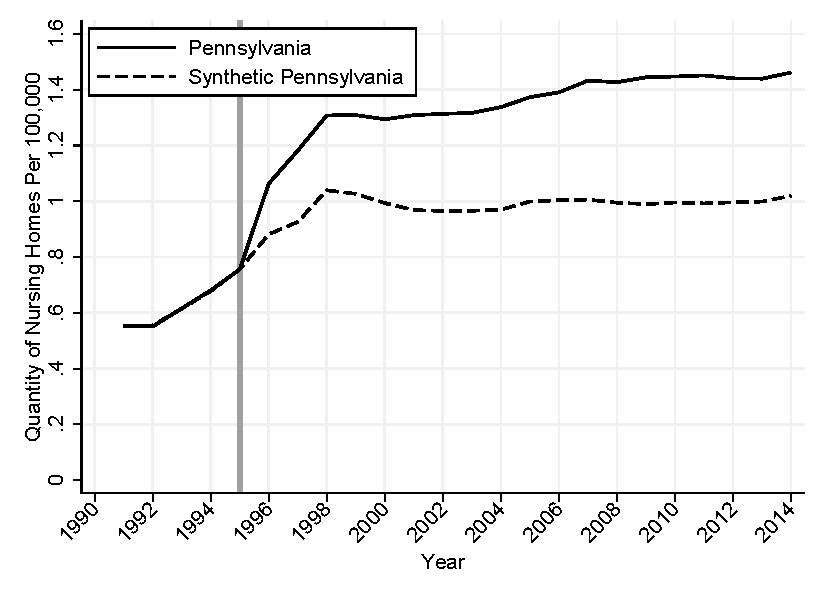
\includegraphics[width=.48\textwidth,keepaspectratio]{q_nursing_homes_Trends_PA.pdf}
    \end{subfigure}\\
    \vspace{.4cm}
    \begin{subfigure}[b]{.48\textwidth} \centering
    \caption{Indiana}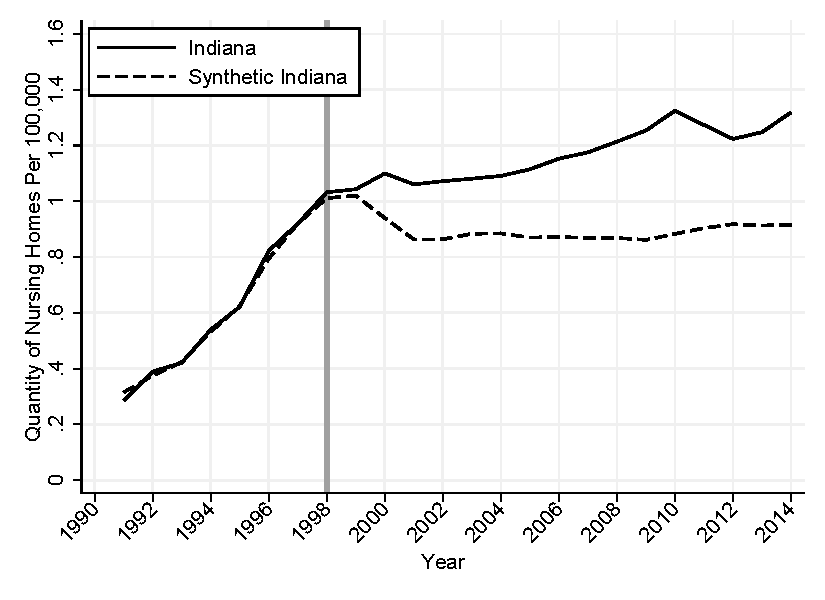
\includegraphics[width=\textwidth,keepaspectratio]{q_nursing_homes_Trends_IN.pdf}
    \end{subfigure}\quad%
    \begin{subfigure}[b]{.48\textwidth} \centering
    \caption{North Dakota}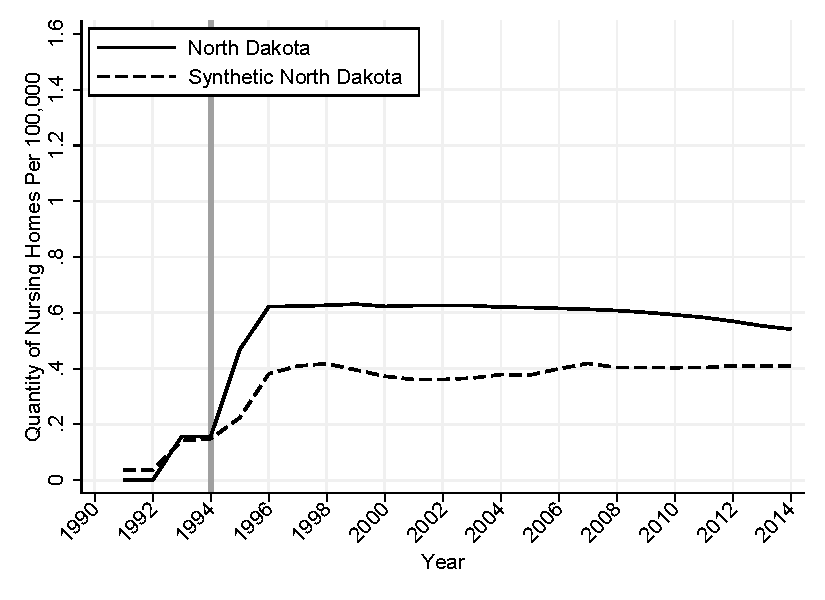
\includegraphics[width=\textwidth,keepaspectratio]{q_nursing_homes_Trends_ND.pdf}
    \end{subfigure}
    \end{center}
    \footnotesize
		\textit{Notes}: This figure shows trends over time in the quantity of nursing homes per 100,000 in PA, IN, and ND and their respective synthetic controls. The vertical lines represent the year in which each state dropped NH-CON regulations. Data source: 1991-2014 Centers for Medicare and Medicaid Services’ (CMS) Provider of Services files.
\end{figure}
\clearpage


\newpage
\begin{figure}[t]
	\begin{center}
	\caption{\label{fig:q_nursing_homes_gaps} \centering Year-Specific Effects of Dropping NH-CON on the Quantity of Nursing Homes Per 100,000 ($\hat{\alpha}_{1t}$)}
    \begin{subfigure}[b]{\textwidth} \centering
    \caption{Pennsylvania}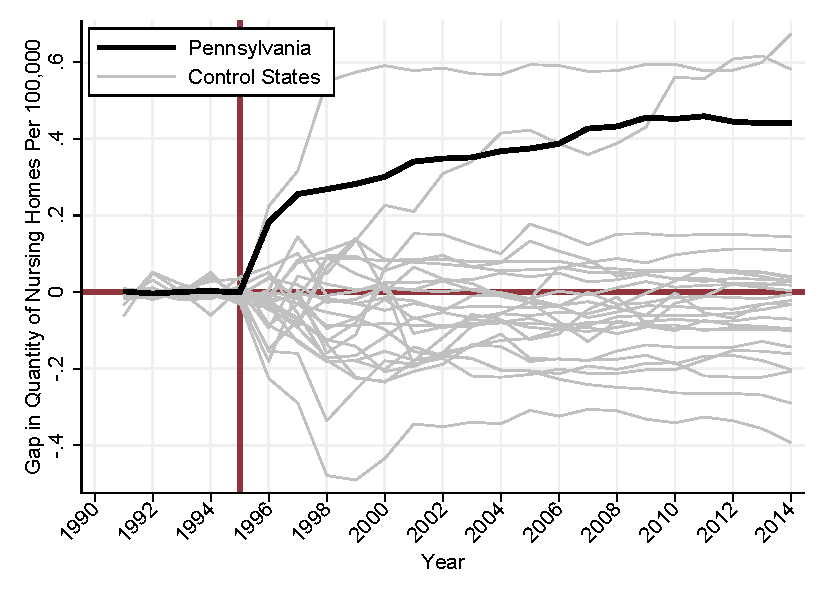
\includegraphics[width=.48\textwidth,keepaspectratio]{q_nursing_homes_Gaps_with_Placebos_20_PA.pdf}
    \end{subfigure}\\
    \vspace{.4cm}
    \begin{subfigure}[b]{.48\textwidth} \centering
    \caption{Indiana}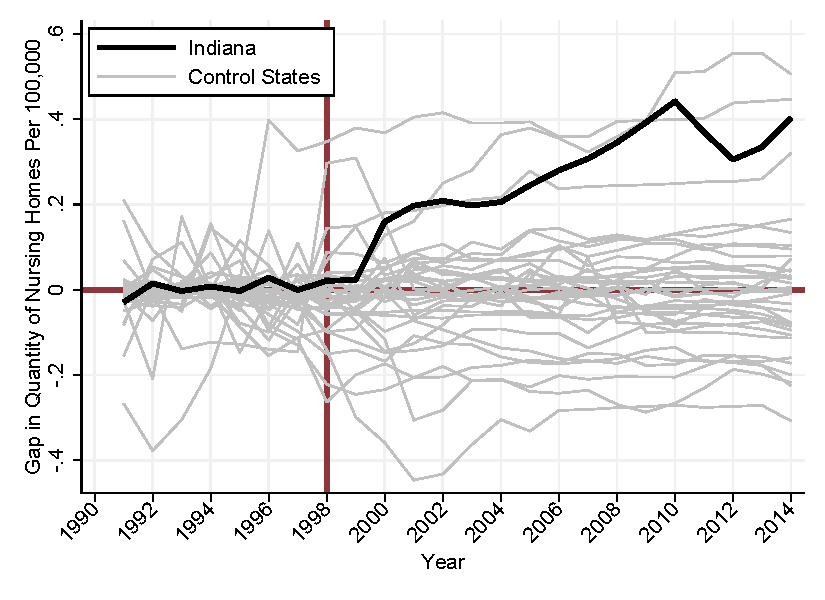
\includegraphics[width=\textwidth,keepaspectratio]{q_nursing_homes_Gaps_with_Placebos_20_IN.pdf}
    \end{subfigure}\quad%
    \begin{subfigure}[b]{.48\textwidth} \centering
    \caption{North Dakota}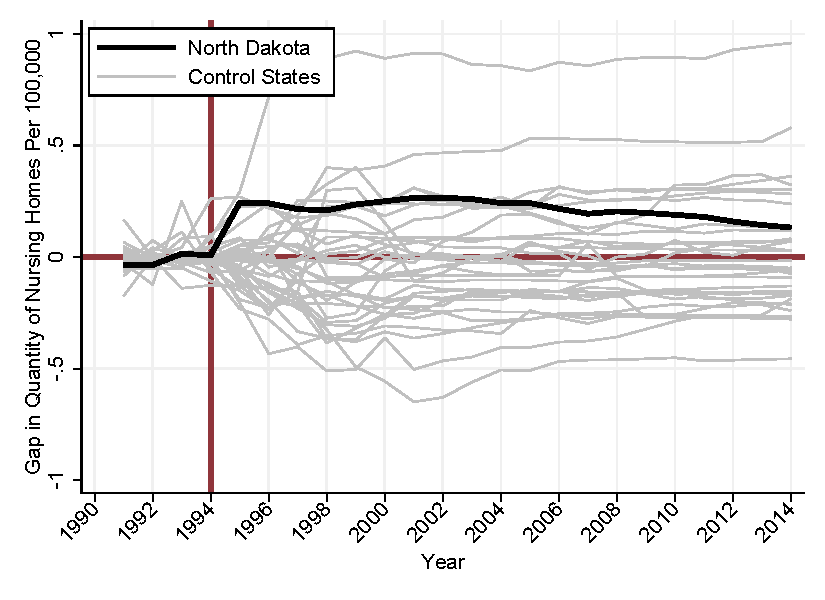
\includegraphics[width=\textwidth,keepaspectratio]{q_nursing_homes_Gaps_with_Placebos_20_ND.pdf}
    \end{subfigure}
    \end{center}
    \footnotesize
		\textit{Notes}: The solid black lines in this figure represent the year-specific effects of dropping NH-CON regulations on the quantity of nursing homes per 100,000 in PA, IN, and ND ($\hat{\alpha}_{1t}$ from equation (\ref{eq:year_spec_effect})). The light gray lines represent the year-specific placebo effects for the states in the donor pool of potential control states. We only show states that have a relatively good fit in the pre-treatment period by dropping states from the figure with an $RMSPE_i^{pre}$ more than twenty times the $RMSPE_i^{pre}$ of the treated states \citep{abadie2010synthetic}. The vertical lines represent the year in which each state dropped NH-CON regulations. Data source: 1980-2014 National Health Expenditure Accounts (NHEA).
\end{figure}
\clearpage


\newpage
\begin{figure}[t]
	\begin{center}
	\caption{\label{fig:q_nursing_home_beds_trends} \centering Trends in the Quantity of Nursing Home Beds Per 100,000}
    \begin{subfigure}[b]{\textwidth} \centering
    \caption{Pennsylvania}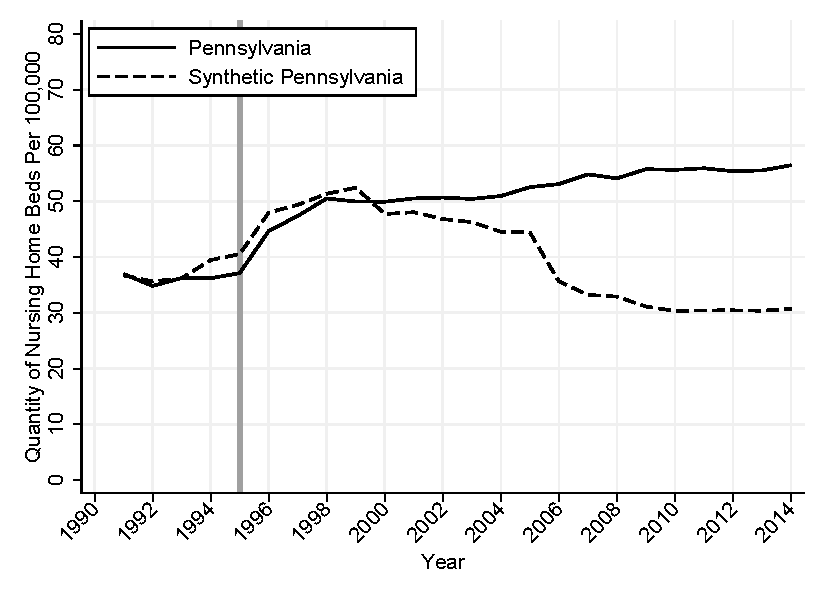
\includegraphics[width=.48\textwidth,keepaspectratio]{q_nursing_home_beds_Trends_PA.pdf}
    \end{subfigure}\\
    \vspace{.4cm}
    \begin{subfigure}[b]{.48\textwidth} \centering
    \caption{Indiana}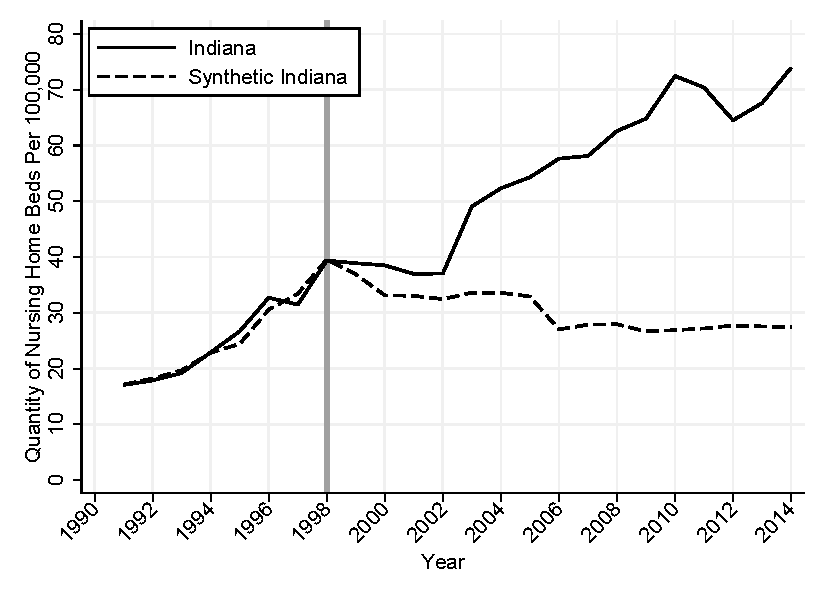
\includegraphics[width=\textwidth,keepaspectratio]{q_nursing_home_beds_Trends_IN.pdf}
    \end{subfigure}\quad%
    \begin{subfigure}[b]{.48\textwidth} \centering
    \caption{North Dakota}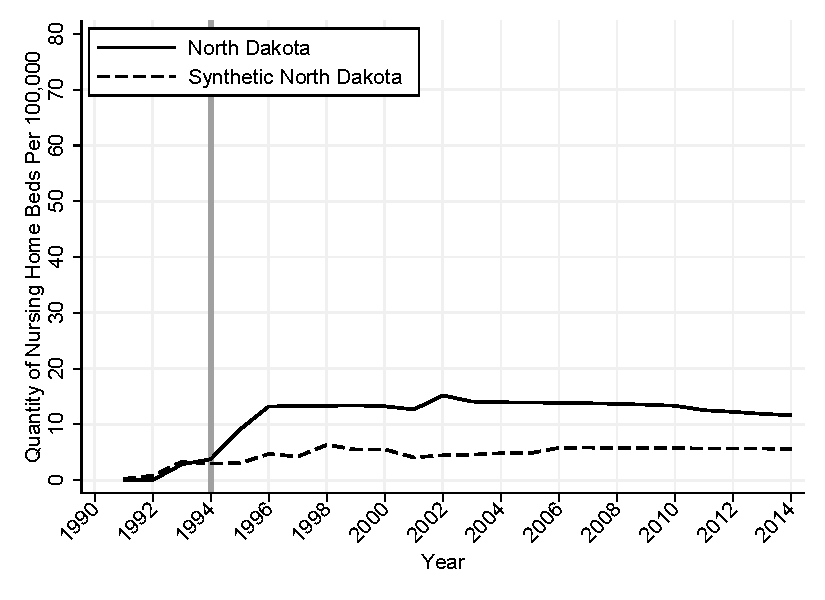
\includegraphics[width=\textwidth,keepaspectratio]{q_nursing_home_beds_Trends_ND.pdf}
    \end{subfigure}
    \end{center}
    \footnotesize
		\textit{Notes}: This figure shows trends over time in the quantity of nursing home beds per 100,000 in PA, IN, and ND and their respective synthetic controls. The vertical lines represent the year in which each state dropped NH-CON regulations. Data source: 1991-2014 Centers for Medicare and Medicaid Services’ (CMS) Provider of Services files.
\end{figure}
\clearpage


\newpage
\begin{figure}[t]
	\begin{center}
	\caption{\label{fig:q_nursing_home_beds_gaps} \centering Year-Specific Effects of Dropping NH-CON on the Quantity of Nursing Home Beds Per 100,000 ($\hat{\alpha}_{1t}$)}
    \begin{subfigure}[b]{\textwidth} \centering
    \caption{Pennsylvania}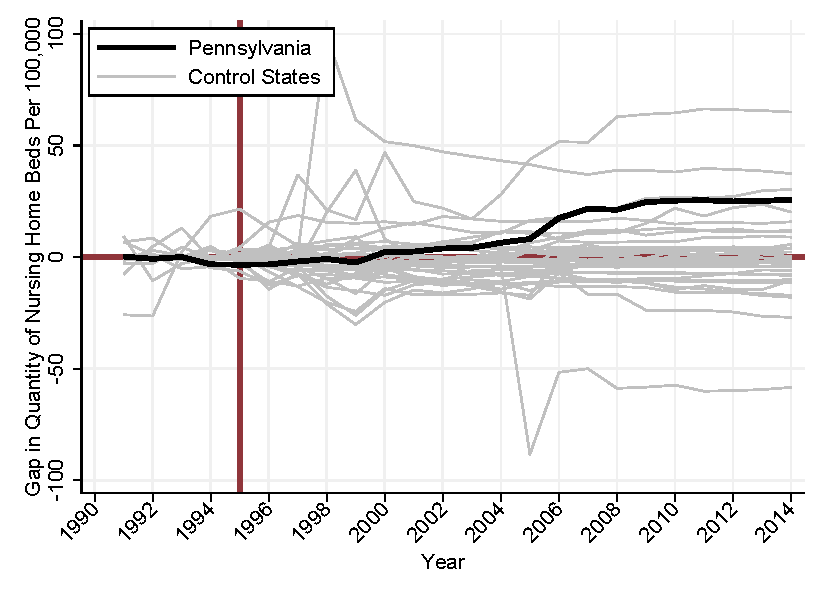
\includegraphics[width=.48\textwidth,keepaspectratio]{q_nursing_home_beds_Gaps_with_Placebos_20_PA.pdf}
    \end{subfigure}\\
    \vspace{.4cm}
    \begin{subfigure}[b]{.48\textwidth} \centering
    \caption{Indiana}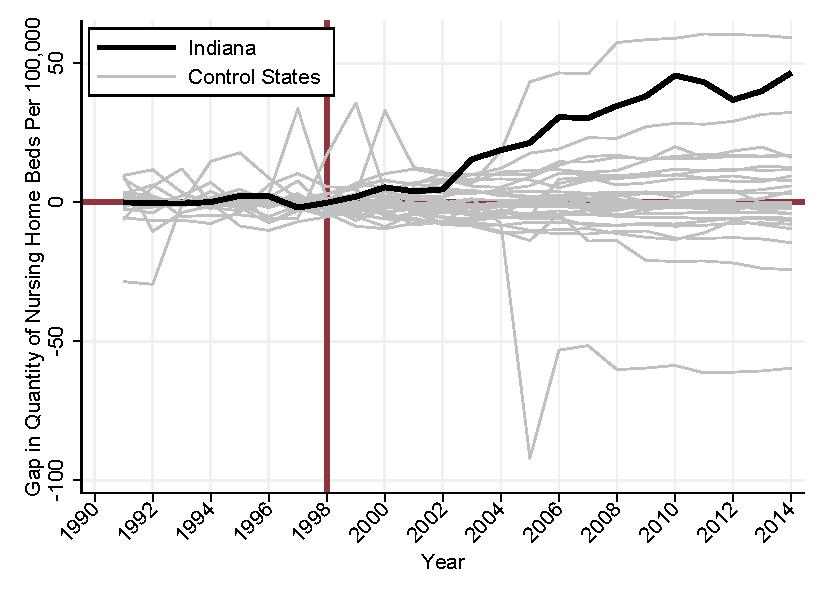
\includegraphics[width=\textwidth,keepaspectratio]{q_nursing_home_beds_Gaps_with_Placebos_20_IN.pdf}
    \end{subfigure}\quad%
    \begin{subfigure}[b]{.48\textwidth} \centering
    \caption{North Dakota}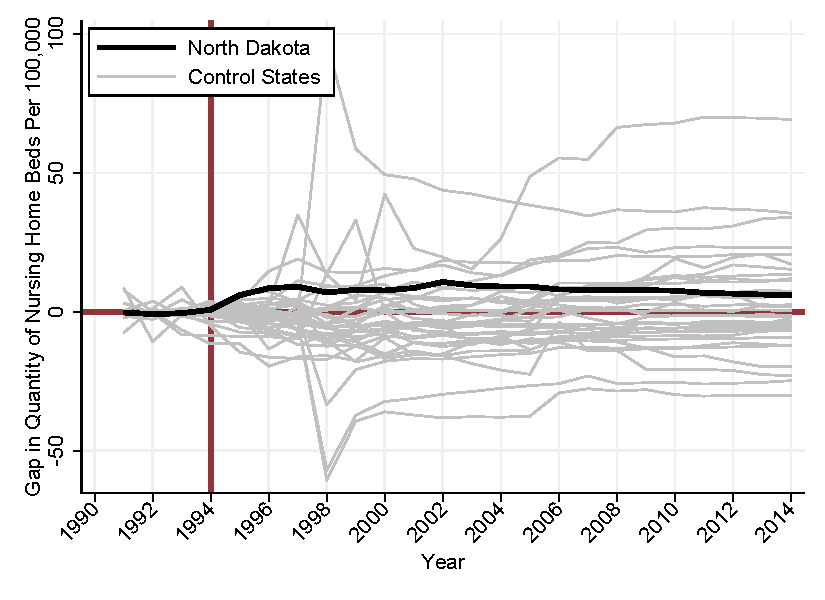
\includegraphics[width=\textwidth,keepaspectratio]{q_nursing_home_beds_Gaps_with_Placebos_20_ND.pdf}
    \end{subfigure}
    \end{center}
    \footnotesize
		\textit{Notes}: The solid black lines in this figure represent the year-specific effects of dropping NH-CON regulations on the quantity of nursing home beds per 100,000 in PA, IN, and ND ($\hat{\alpha}_{1t}$ from equation (\ref{eq:year_spec_effect})). The light gray lines represent the year-specific placebo effects for the states in the donor pool of potential control states. We only show states that have a relatively good fit in the pre-treatment period by dropping states from the figure with an $RMSPE_i^{pre}$ more than twenty times the $RMSPE_i^{pre}$ of the treated states \citep{abadie2010synthetic}. The vertical lines represent the year in which each state dropped NH-CON regulations. Data source: 1980-2014 National Health Expenditure Accounts (NHEA).
\end{figure}
\clearpage

\newpage
\begin{figure}[t]
	\begin{center}
	\caption{\label{fig:tot_exp_trends} \centering Trends in Total Nursing Home Expenditure Per Capita}
    \begin{subfigure}[b]{\textwidth} \centering
    \caption{Pennsylvania}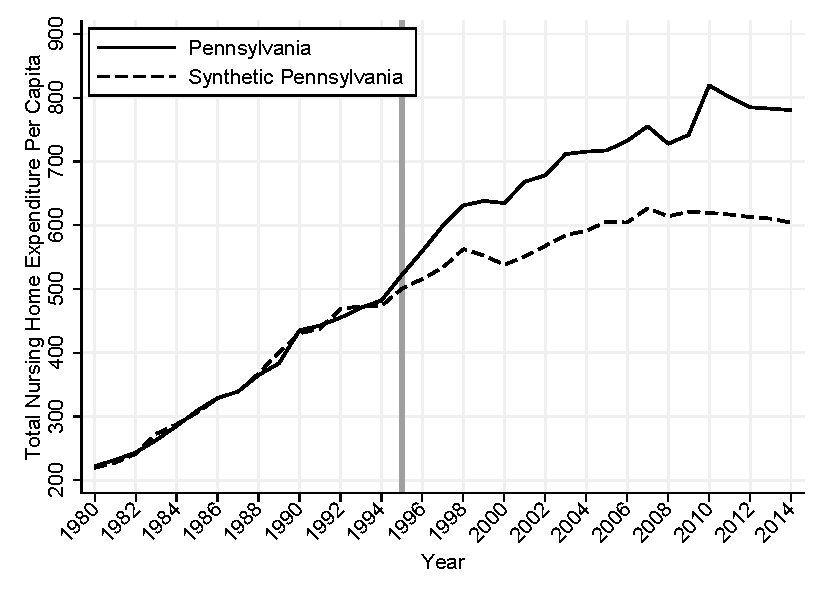
\includegraphics[width=.48\textwidth,keepaspectratio]{nursing_home_tot_exp_Trends_PA.pdf}
    \end{subfigure}\\
    \vspace{.4cm}
    \begin{subfigure}[b]{.48\textwidth} \centering
    \caption{Indiana}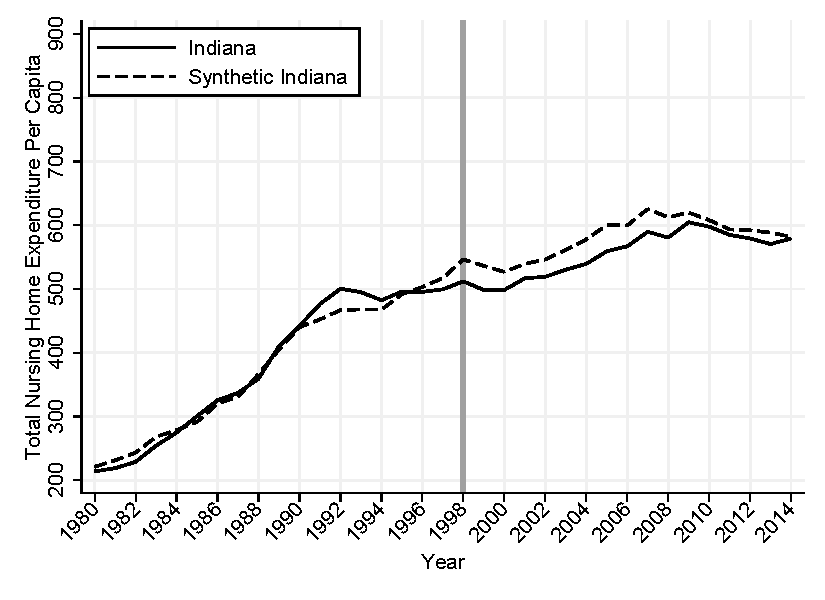
\includegraphics[width=\textwidth,keepaspectratio]{nursing_home_tot_exp_Trends_IN.pdf}
    \end{subfigure}\quad%
    \begin{subfigure}[b]{.48\textwidth} \centering
    \caption{North Dakota}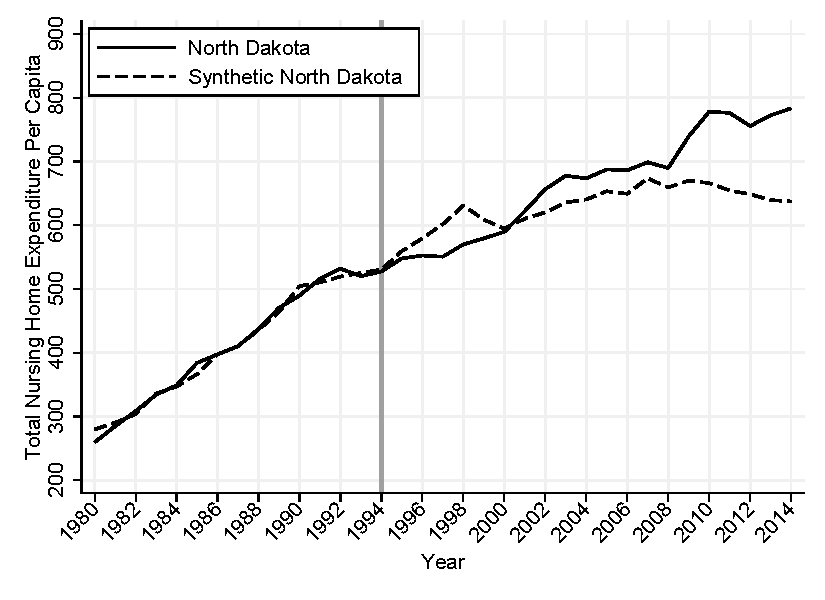
\includegraphics[width=\textwidth,keepaspectratio]{nursing_home_tot_exp_Trends_ND.pdf}
    \end{subfigure}
    \end{center}
    \footnotesize
		\textit{Notes}: This figure shows trends over time in total nursing home expenditure per capita in PA, IN, and ND and their respective synthetic controls. The vertical lines represent the year in which each state dropped NH-CON regulations. Data source: 1980-2014 National Health Expenditure Accounts (NHEA).
\end{figure}
\clearpage



\newpage
\begin{figure}[t]
	\begin{center}
	\caption{\label{fig:tot_exp_gaps} \centering Year-Specific Effects of Dropping NH-CON on Total Expenditure Per Capita ($\hat{\alpha}_{1t}$)}
    \begin{subfigure}[b]{\textwidth} \centering
    \caption{Pennsylvania}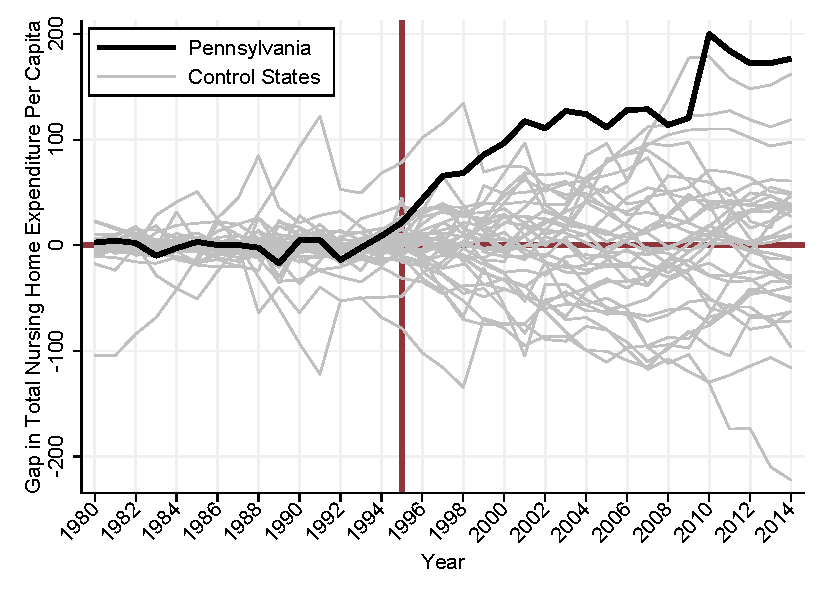
\includegraphics[width=.48\textwidth,keepaspectratio]{nursing_home_tot_exp_Gaps_with_Placebos_20_PA.pdf}
    \end{subfigure}\\
    \vspace{.4cm}
    \begin{subfigure}[b]{.48\textwidth} \centering
    \caption{Indiana}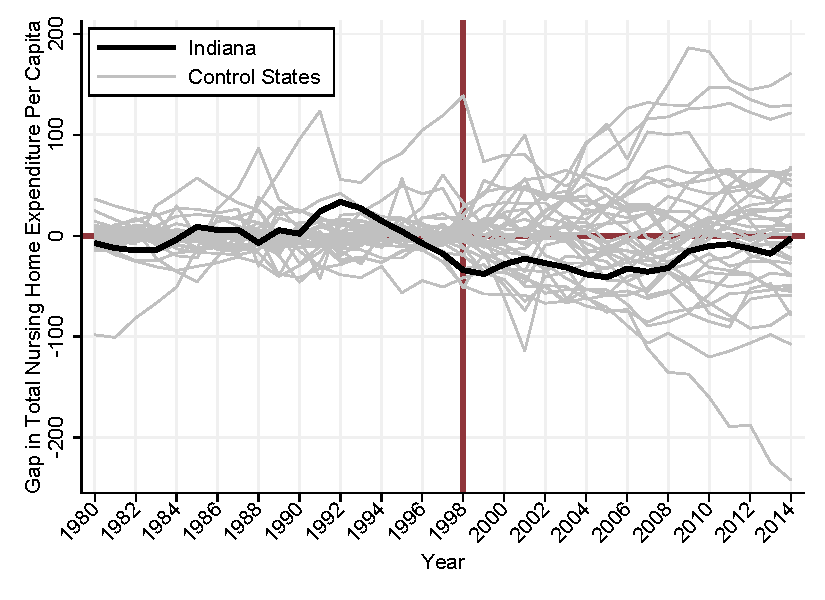
\includegraphics[width=\textwidth,keepaspectratio]{nursing_home_tot_exp_Gaps_with_Placebos_20_IN.pdf}
    \end{subfigure}\quad%
    \begin{subfigure}[b]{.48\textwidth} \centering
    \caption{North Dakota}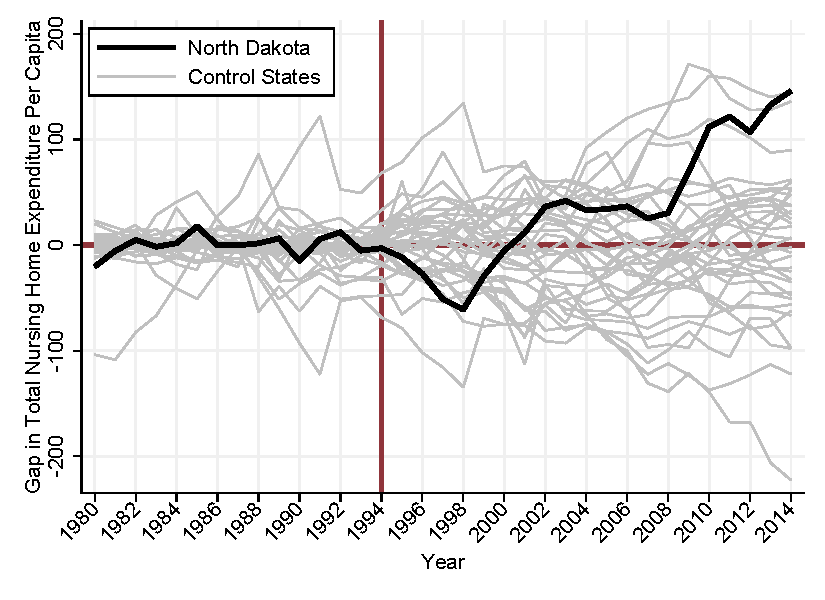
\includegraphics[width=\textwidth,keepaspectratio]{nursing_home_tot_exp_Gaps_with_Placebos_20_ND.pdf}
    \end{subfigure}
    \end{center}
    \footnotesize
		\textit{Notes}: The solid black lines in this figure represent the year-specific effects of dropping NH-CON regulations on total nursing home expenditure per capita in PA, IN, and ND ($\hat{\alpha}_{1t}$ from equation (\ref{eq:year_spec_effect})). The light gray lines represent the year-specific placebo effects for the states in the donor pool of potential control states. We only show states that have a relatively good fit in the pre-treatment period by dropping states from the figure with an $RMSPE_i^{pre}$ more than twenty times the $RMSPE_i^{pre}$ of the treated states \citep{abadie2010synthetic}. The vertical lines represent the year in which each state dropped NH-CON regulations. Data source: 1980-2014 National Health Expenditure Accounts (NHEA).
\end{figure}
\clearpage



\newpage
\begin{figure}[t]
	\begin{center}
	\caption{\label{fig:medicaid_exp_trends} \centering Trends in Nursing Home Medicaid Expenditure Per Capita}
    \begin{subfigure}[b]{\textwidth} \centering
    \caption{Pennsylvania}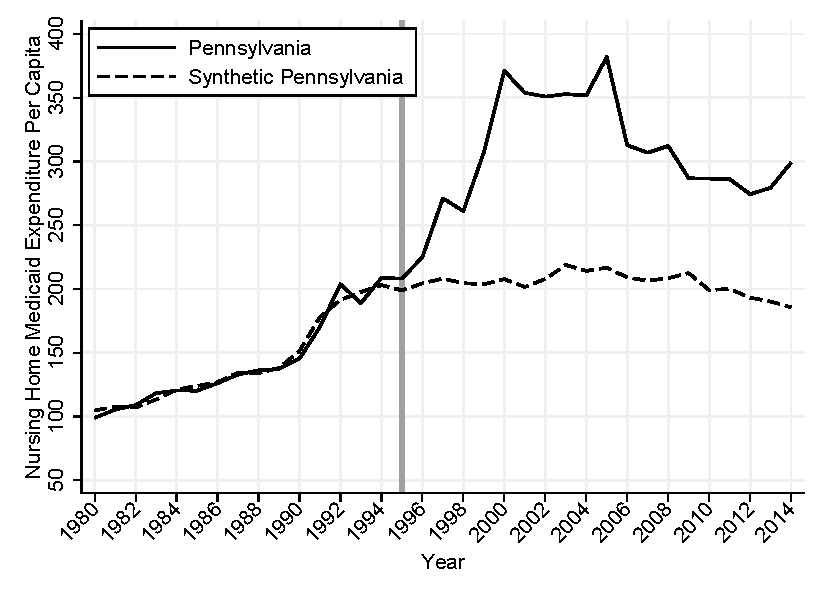
\includegraphics[width=.48\textwidth,keepaspectratio]{nursing_home_medicaid_exp_Trends_PA.pdf}
    \end{subfigure}\\
    \vspace{.4cm}
    \begin{subfigure}[b]{.48\textwidth} \centering
    \caption{Indiana}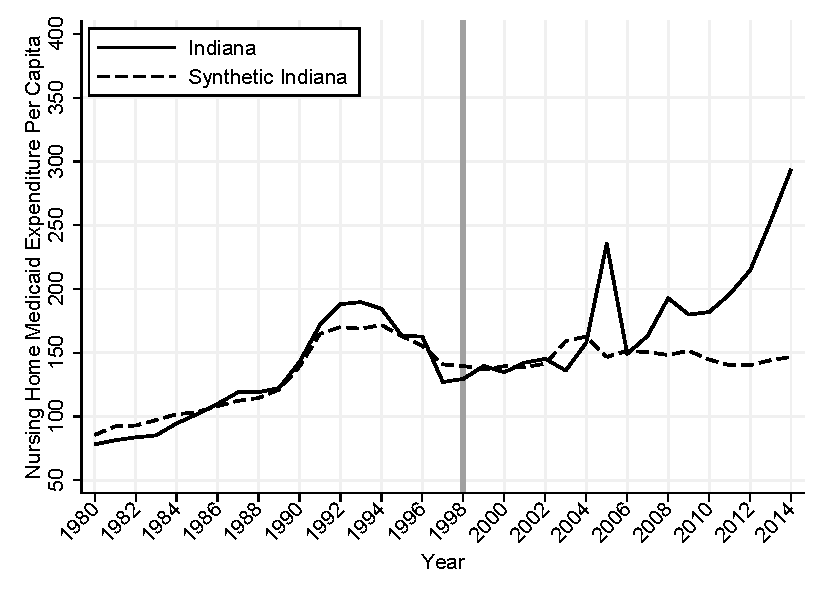
\includegraphics[width=\textwidth,keepaspectratio]{nursing_home_medicaid_exp_Trends_IN.pdf}
    \end{subfigure}\quad%
    \begin{subfigure}[b]{.48\textwidth} \centering
    \caption{North Dakota}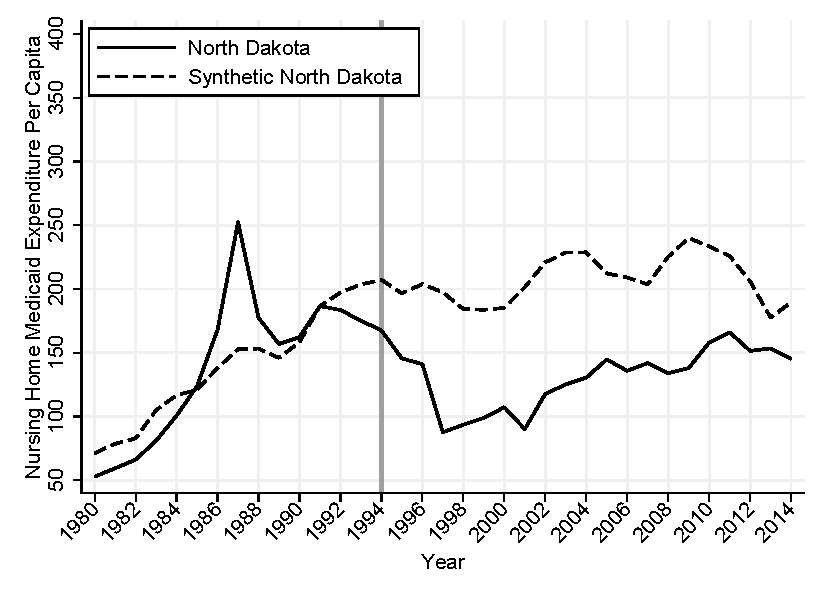
\includegraphics[width=\textwidth,keepaspectratio]{nursing_home_medicaid_exp_Trends_ND.pdf}
    \end{subfigure}
    \end{center}
    \footnotesize
		\textit{Notes}: This figure shows trends over time in nursing home medicaid expenditure per capita in PA, IN, and ND and their respective synthetic controls. The vertical lines represent the year in which each state dropped NH-CON regulations. Data source: 1980-2014 National Health Expenditure Accounts (NHEA).
\end{figure}
\clearpage



\newpage
\begin{figure}[t]
	\begin{center}
	\caption{\label{fig:medicaid_exp_gaps} \centering Year-Specific Effects of Dropping NH-CON on Medicaid Expenditure Per Capita ($\hat{\alpha}_{1t}$)}
    \begin{subfigure}[b]{\textwidth} \centering
    \caption{Pennsylvania}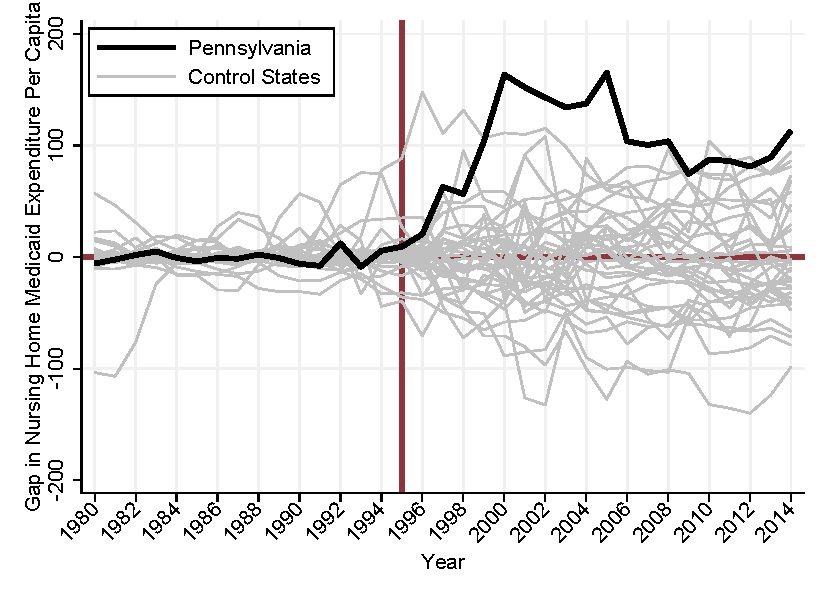
\includegraphics[width=.48\textwidth,keepaspectratio]{nursing_home_medicaid_exp_Gaps_with_Placebos_20_PA.pdf}
    \end{subfigure}\\
    \vspace{.4cm}
    \begin{subfigure}[b]{.48\textwidth} \centering
    \caption{Indiana}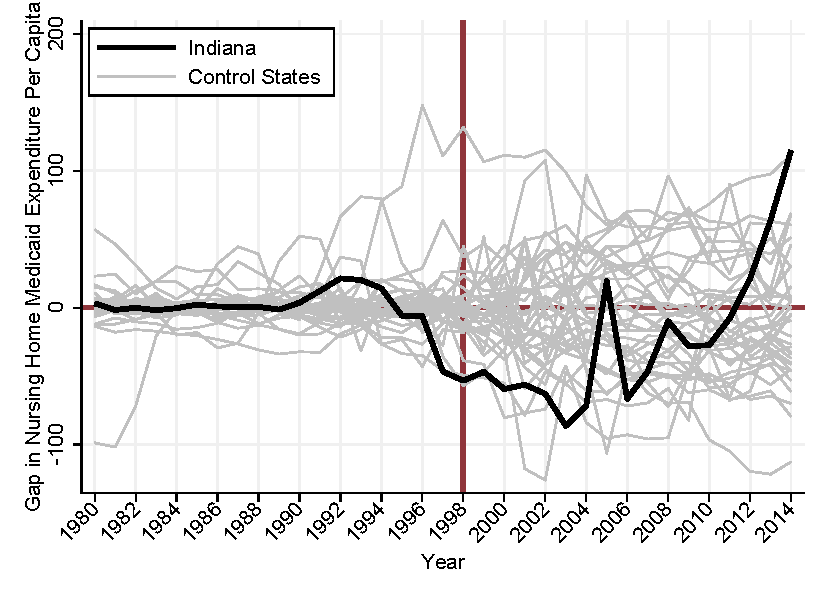
\includegraphics[width=\textwidth,keepaspectratio]{nursing_home_medicaid_exp_Gaps_with_Placebos_20_IN.pdf}
    \end{subfigure}\quad%
    \begin{subfigure}[b]{.48\textwidth} \centering
    \caption{North Dakota}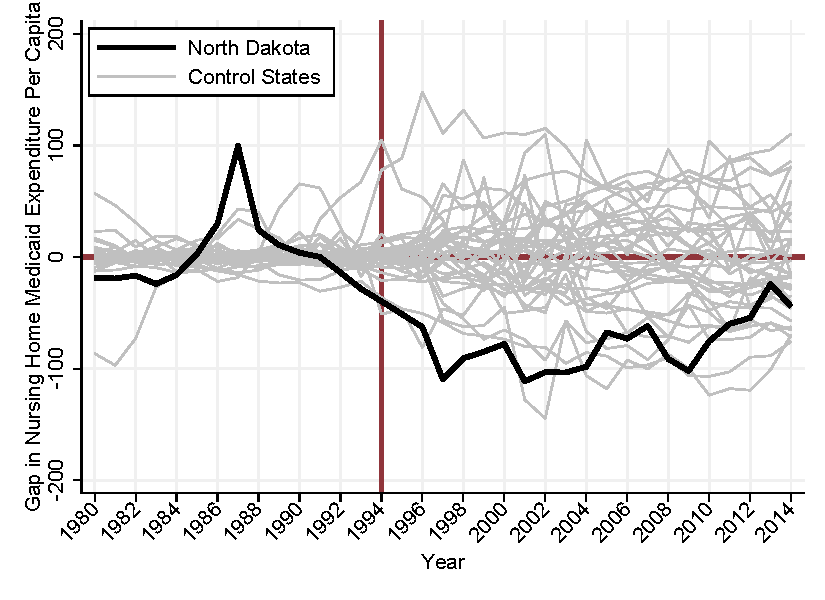
\includegraphics[width=\textwidth,keepaspectratio]{nursing_home_medicaid_exp_Gaps_with_Placebos_20_ND.pdf}
    \end{subfigure}
    \end{center}
    \footnotesize
		\textit{Notes}: The solid black lines in this figure represent the year-specific effects of dropping NH-CON regulations on nursing home medicaid expenditure per capita in PA, IN, and ND ($\hat{\alpha}_{1t}$ from equation (\ref{eq:year_spec_effect})). The light gray lines represent the year-specific placebo effects for the states in the donor pool of potential control states. We only show states that have a relatively good fit in the pre-treatment period by dropping states from the figure with an $RMSPE_i^{pre}$ more than twenty times the $RMSPE_i^{pre}$ of the treated states \citep{abadie2010synthetic}. The vertical lines represent the year in which each state dropped NH-CON regulations. Data source: 1980-2014 National Health Expenditure Accounts (NHEA).
\end{figure}
\clearpage

	


\end{document}